\documentclass[a4paper,ngerman]{scrartcl}

\usepackage{amsmath}
\usepackage{amsfonts}
\usepackage{amssymb}
\usepackage[utf8]{inputenc}
\usepackage{graphicx}
\usepackage[ngerman]{babel}
\usepackage{hyperref}
\usepackage{float}
\usepackage{caption}
\usepackage{subcaption}
\usepackage{multirow}  %for tables
\usepackage{icomma} % Handle german comma as decimal point in numbers
\usepackage{units,siunitx} % Write units with correct spacing
\usepackage{upgreek} % provide non-italic greek letters
\usepackage{url}
\usepackage{booktabs}
%\usepackage{subfig}

% Formatting of table & figure captions
\captionsetup{font={sf,footnotesize},labelfont=bf,textfont=sl,skip=6pt}
\setlength{\abovecaptionskip}{6pt}
\setlength{\belowcaptionskip}{0pt}

\title{Landéfaktor\\Versuchsauswertung}
\date{\today}
\author{Michel Rausch, Michael Eliachevitch}

\begin{document}

\maketitle
\tableofcontents
\newpage

\section{Zeitkalibrierung}

Ein Funktionsgenerator wurde an den Starteingang des TAC geschlossen, sowie über Verzögerungsglieder an des Stoppeingang. Diese wurden hinzugeschaltet, um die Zeitverzögerung in bekannten Schritten von $\SI{1}{\nano \second}$ zu erhöhen. Das zugehörige Peaks war scharf gegenüber des Abstandes, sodass die Messungen in einer einzelnen Grafik, Abb. \ref{fig:zeitkalibrierung_hist}, auswerten ließen. Die Nummer des Kanals steigt mit der zugehörigen Verzögerung. 

\begin{figure}[tb!]
\centering
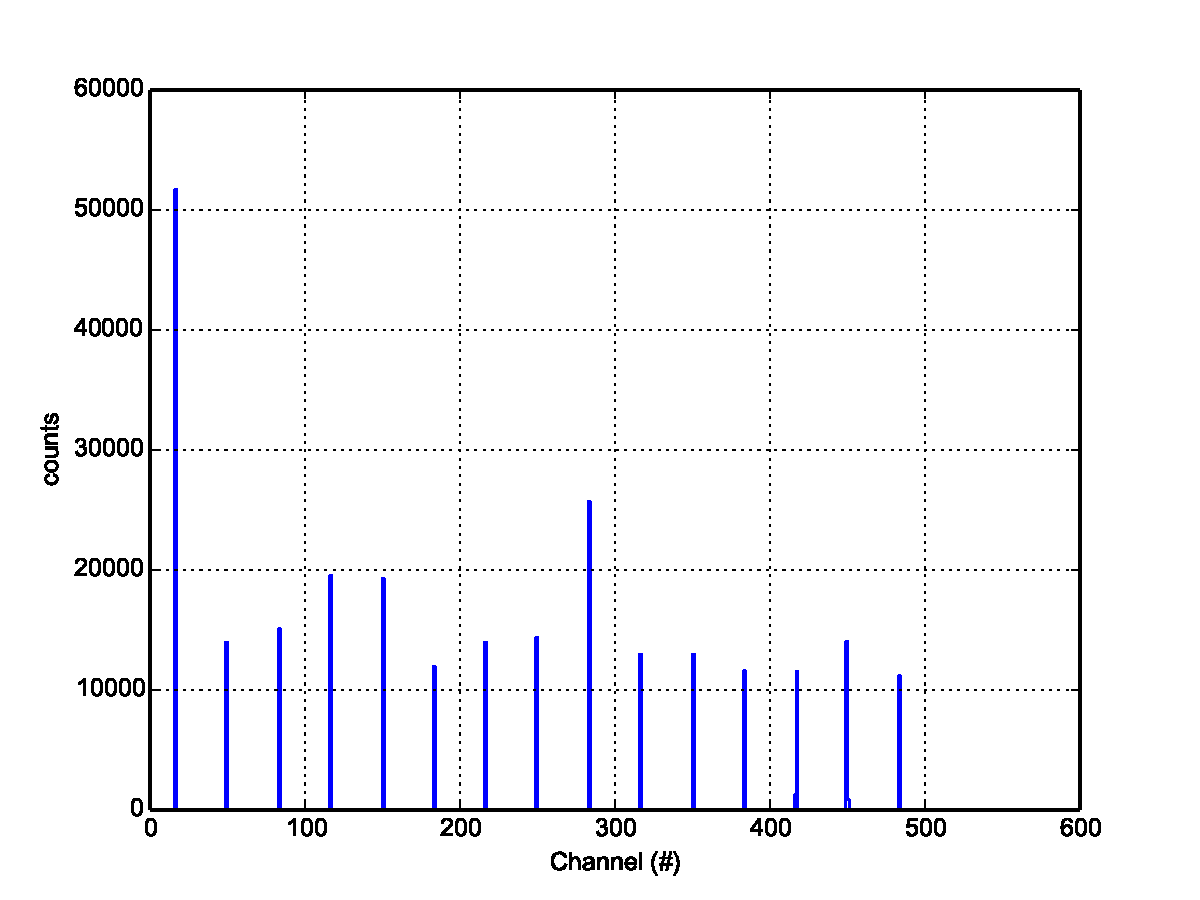
\includegraphics[width=0.7\textwidth]{abbildungen/zeitkalibrierung_hist.pdf}
\caption[Daten zur Zeitkalibrierung]{\textbf{Daten zur Zeitkalibrierung.} Die gezeigten Peaks gehören zu unterschiedlichen Verzögerungen. Da sie sich signifikant unterscheiden, ließen sie sich in einer Grafik auswerten. Die Verzögerung wird von dem Peak am weitesten links nach rechts schrittweise um $\SI{1}{\nano \second}$ größer.}
\label{fig:zeitkalibrierung_hist}
\end{figure}


Die Zeit wurde den Kanälen zugewiesen. Mit Python wurde eine lineare Regression durchgeführt. Mit der resultierenden Geradengleichung wurden die Kanäle einer Zeit zugewiesen. Die Regression ist in Abbildung \ref{fig:zeitkalibrierung} gezeigt, das Ergebnis lautet

\begin{equation}
\label{eqn:Zeitkalibrierung}
\frac{\mathrm{Zeit}}{\mathrm{Kanal}} = \SI{0.029978 }{\nano \second} .
\end{equation}


\begin{figure}[tb!]
\centering
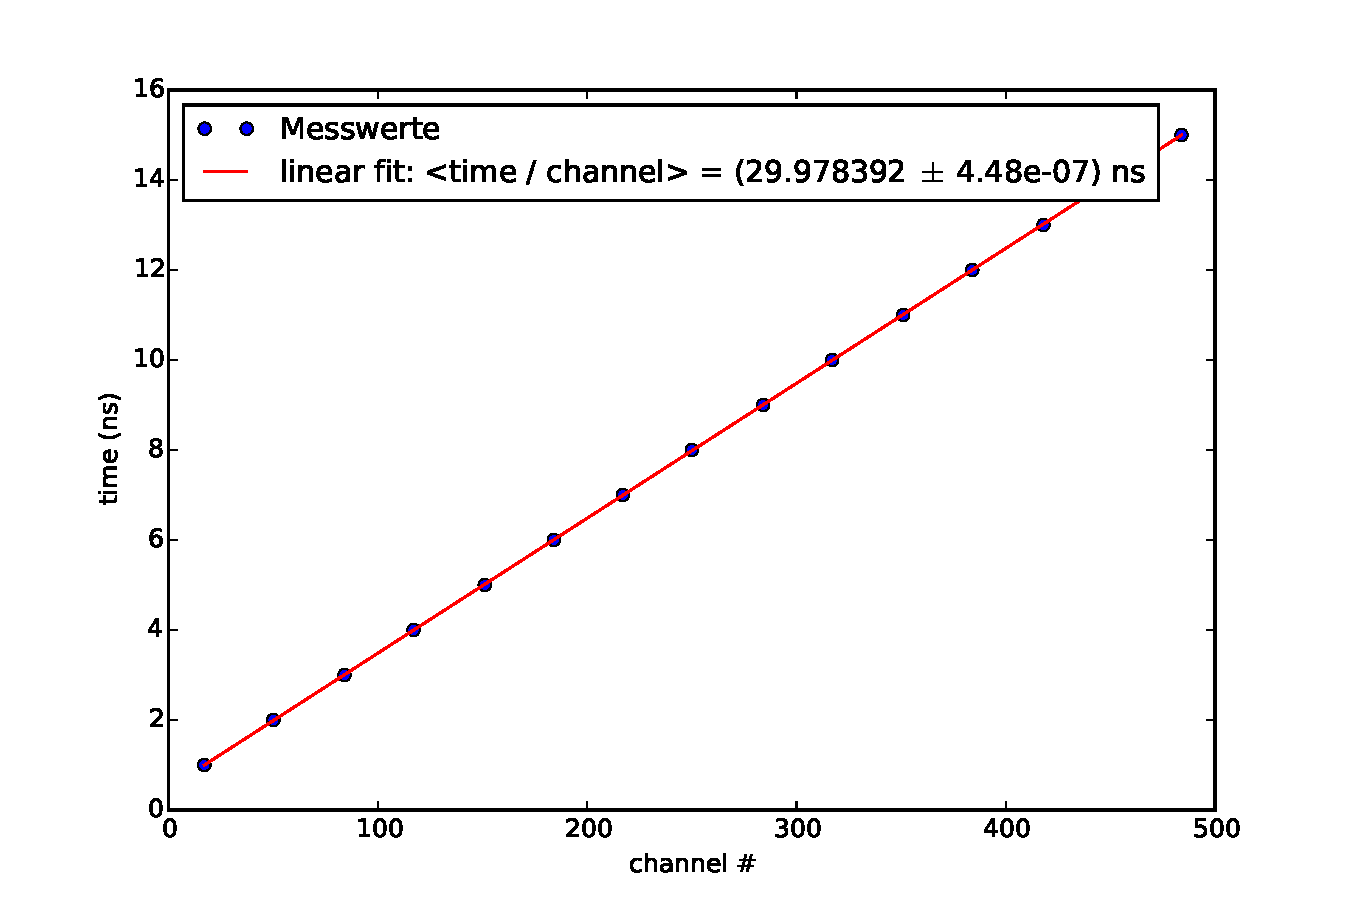
\includegraphics[width=0.7\textwidth]{abbildungen/zeitkalibrierung.pdf}
\caption[Zeitkalibrierung]{\textbf{Zeitkalibrierung.} Mittels eines Pythonscripts wurde ein linearer Fit durchgeführt. Die Kanalnummer des VKAs wird auf der x-Achse aufgetragen, die dazugehörige Verzögerung auf der y-Achse.}
\label{fig:zeitkalibrierung}
\end{figure}

\section{Bestimmung der Lebensdauer des Myons}

\section{Bestimmung des Landéfaktors des Myons}
%Am Besten noch was zu g schreiben, in der Vorbereitung war nicht ausreichend erklärt, was es ist.

\subsection{Bedeutung des Landéfaktors}

\section{Diskussion der Ergebnisse}

\section{Quellen}
\begin{enumerate}
\item Vorbereitungsmappe 
\end{enumerate}



\end{document}
